L'application est conçue selon le \textit{modèle en couche}.

\subsection{Paquetages}
Le modèle en couche consiste à séparer les classes de l'application en trois paquetages (minimum). Dans l'ordre :

\subsubsection{Couche présentation}
La couche \textit{présentation} contient les IHM de l'application. Le code des classes ne contient que ce qui est nécéssaire pour l'agencement et le paramétrage des composants sur la vue.

\subsubsection{Couche contrôle}
La couche \textit{contrôle} contient l'\textit{intelligence} des IHM, c'est à dire ce qu'il doit se passer \textbf{hors} de la vue (dans les bases de données, la RAM etc.) après un clic sur tel ou tel bouton, case à cocher ou tout autre composant.

Cette couche décharge le code des IHM et fait office d'\textit{indirection} entre les vues et le reste de l'application : les IHM ne connaissent que leurs contrôleurs respectifs.

\subsubsection{Couche entité}
La couche \textit{entité} ou \textit{métier} contient la valeur ajouté de l'application, c'est à dire toutes les classes qui offrent le service proposé par l'application.

Dans ce projet tuteuré, les classes métiers sont une pseudo-couche \gls{orm}
\footnote{\label{faux_orm}Les ORM convertissent les données en objets, dans cette application se sont les \textit{conteneurs} des données qui sont convertits en objets.}
qui représentent les tables et les contraintes du SGBD connecté à l'application.
Elles limitent ainsi les accès au SGBD, ce qui augmente les performances de l'application et participent à la génération de code SQL à partir des saisies faites dans les IHM.


\begin{figure}[!h]
  \centering
  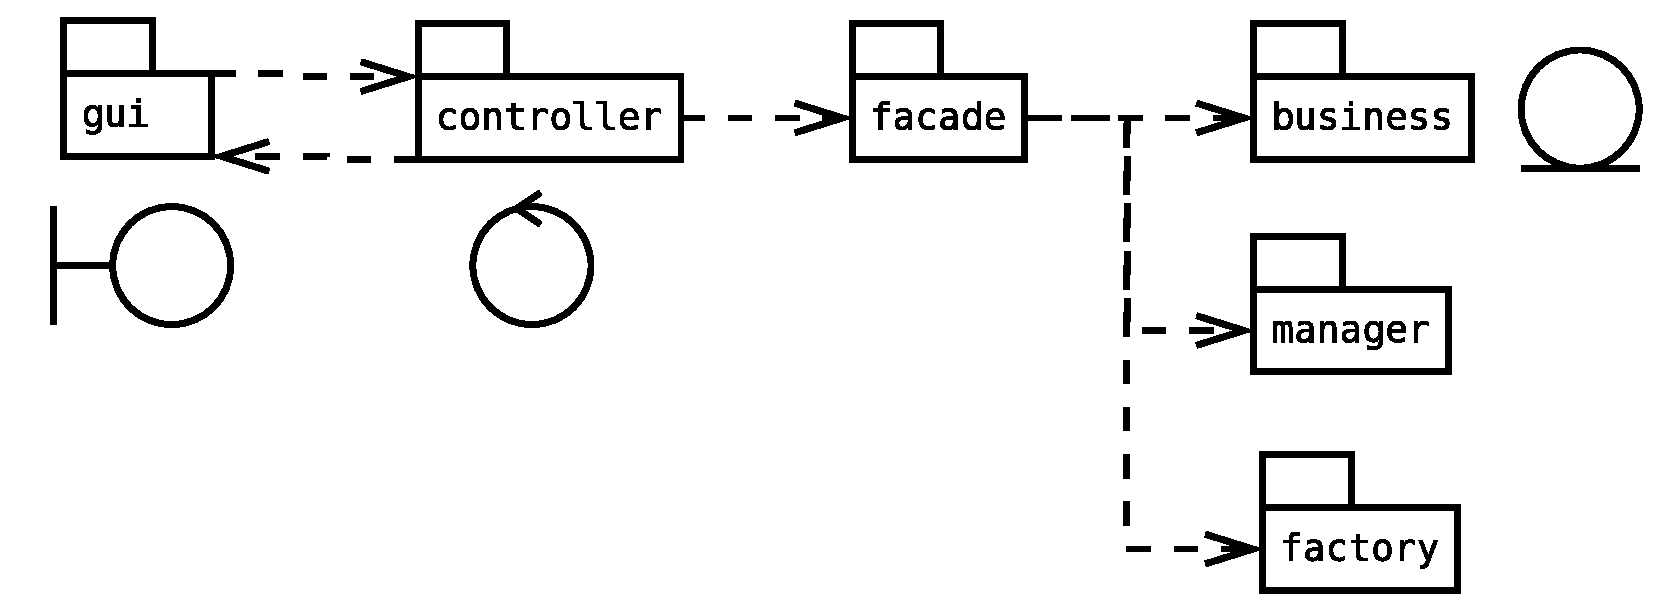
\includegraphics[width=14cm]{images/paquetage.eps}
  \caption{Diagramme de paquetage de l'application.}
  \label{diagramme_de_paquetage_idb}
\end{figure}
